\section{Auswertung}
\label{sec:auswertung}
Im Folgenden werden alle Fehler mit Hilfe der \texttt{python}-Bibliothek
\texttt{uncertainties}\cite{py-uncertainties} berechnet, die eine Gaußsche
Fehlerfortpflanzung implementiert.

\subsection{Untersuchung an amplitudenmodulierten Schwingungen}
\label{subsec:am-auswertung}
Im Folgenden wird das Signal und Frequenzspektrum einer amplitudenmodulierten
Welle betrachtet. Anschließend wird das Signal mit Hilfe eines Ringmodulators,
sowie einer Gleichrichterdiode demoduliert.

\subsubsection{Amplitudenmodulation mit Ringmodulator}
\label{subsubsec:am-ringmodulator}
Das mit Hilfe eines Ringmodulators erzeugte Signal ist in Abbildung
\ref{fig:am-signal} dargestellt.
Das entsprechende Frequenzspektrum wird in Abbildung \ref{fig:am-spektrum}
gezeigt.
\begin{figure}
    \centering
    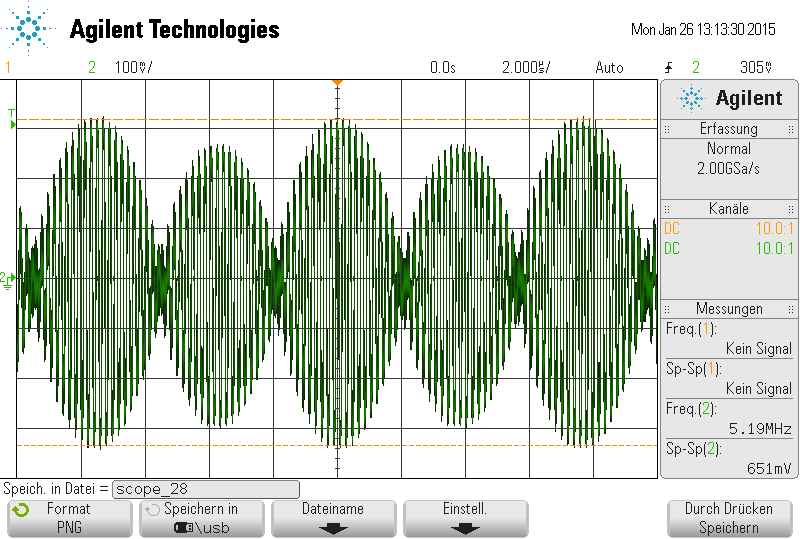
\includegraphics[width=0.8\linewidth]{images/am-signal.png}
    \caption{Amplitudenmoduliertes Signal.}
    \label{fig:am-signal}
\end{figure}
\begin{figure}
    \centering
    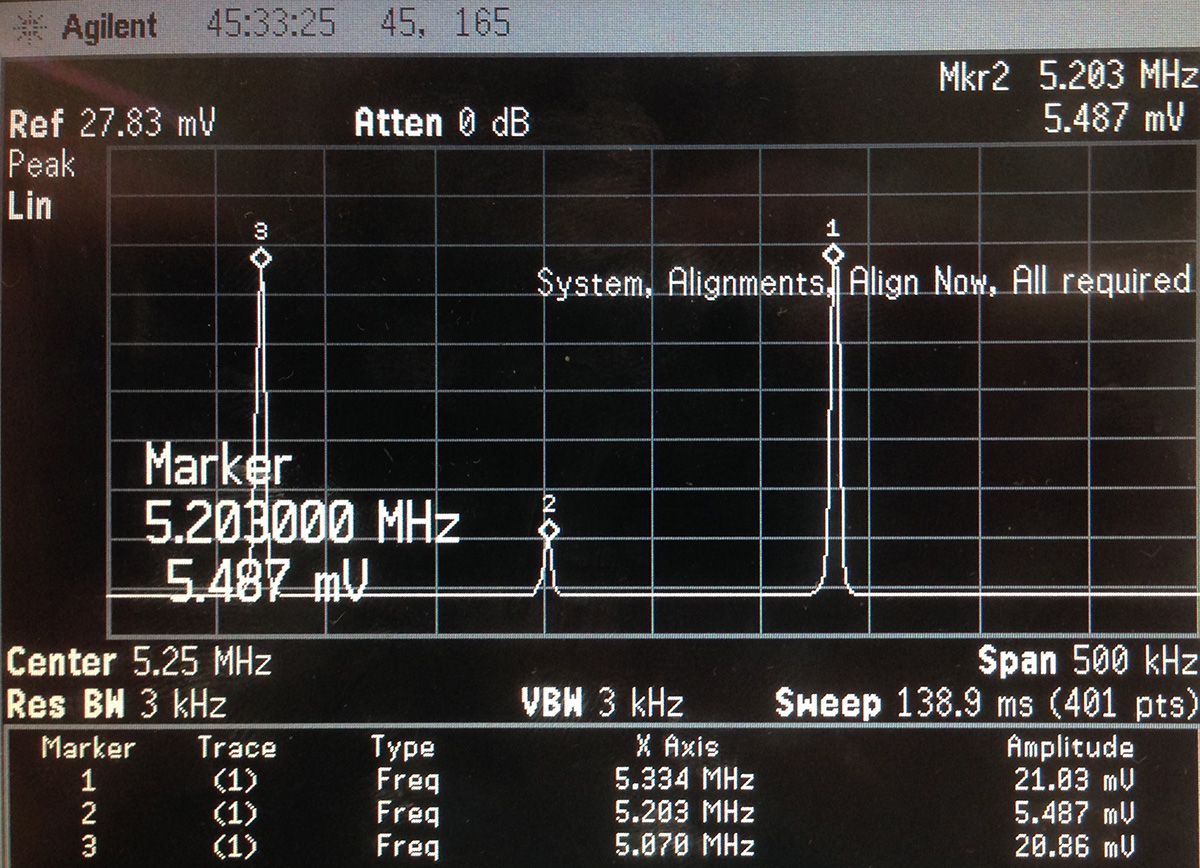
\includegraphics[width=0.8\linewidth]{images/am-spektrum.jpg}
    \caption{
        Frequenzspektrum des AM-Signals im Bereich um die
        Trägerfrequenz.
    }
    \label{fig:am-spektrum}
\end{figure}

\subsubsection{Amplitudenmodulation mit Diode}
\label{subsubsec:am-ringmodulator}
Die Amplitudenmodulation mit Hilfe einer Diode liefert das in Abbildung
\ref{fig:am-diode-signal}, beziehungsweise \ref{fig:am-diode-spektrum}
dargestellte Signal und Spektrum. Die Oberwellen der Trägerfrequenz bei
$2\omega_\text{T} = \SI{10.34}{\mega\hertz}$ und
$3\omega_\text{T} = \SI{15.53}{\mega\hertz}$ treten auf, weil XXX.
Sie sind in Abbildung \ref{fig:am-diode-oberwellen}

Der Modulationsgrad $m$ beträgt mit einer maximalen Schwebungsamplitude
von $U_\text{T}(1+m)=\SI{99.5}{\milli\volt}$ und einer minimalen Amplitude
von $U_\text{T}(1-m)=\SI{50.0}{\milli\volt}$
\begin{equation*}
    m_1 = \input{build/m1.tex}\,.
\end{equation*}
Mit Betrachtung des Frequenzspektrums ergibt sich bei einer Trägerfrequenz
$\omega_\text{T} = \SI{5.207}{\mega\hertz}$ und Seitenfrequenzen bei
$\omega_\text{T} + \omega_\text{M} = \SI{5.338}{\mega\hertz}$ und
$\omega_\text{T} - \omega_\text{M} = \SI{5.074}{\mega\hertz}$, sowie
entsprechenden Amplituden von $U_\text{T} = \SI{4.7+-0.1}{\milli\volt}$,
$U_1 = \SI{1.57+-0.01}{\milli\volt}$ und $U_2 = \SI{1.56+-0.01}{\milli\volt}$
der Modulationsgrad
\begin{equation*}
    m_2 = \input{build/m2.tex}\,.
\end{equation*}
\begin{figure}
    \centering
    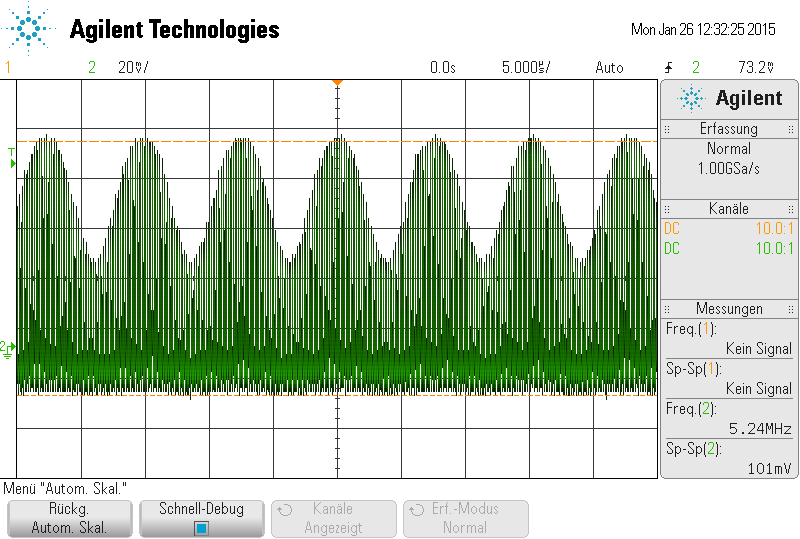
\includegraphics[width=0.8\linewidth]{images/am-diode-signal.png}
    \caption{Mit Hilfe einer Diode moduliertes Signal.}
    \label{fig:am-diode-signal}
\end{figure}
\begin{figure}
    \centering
    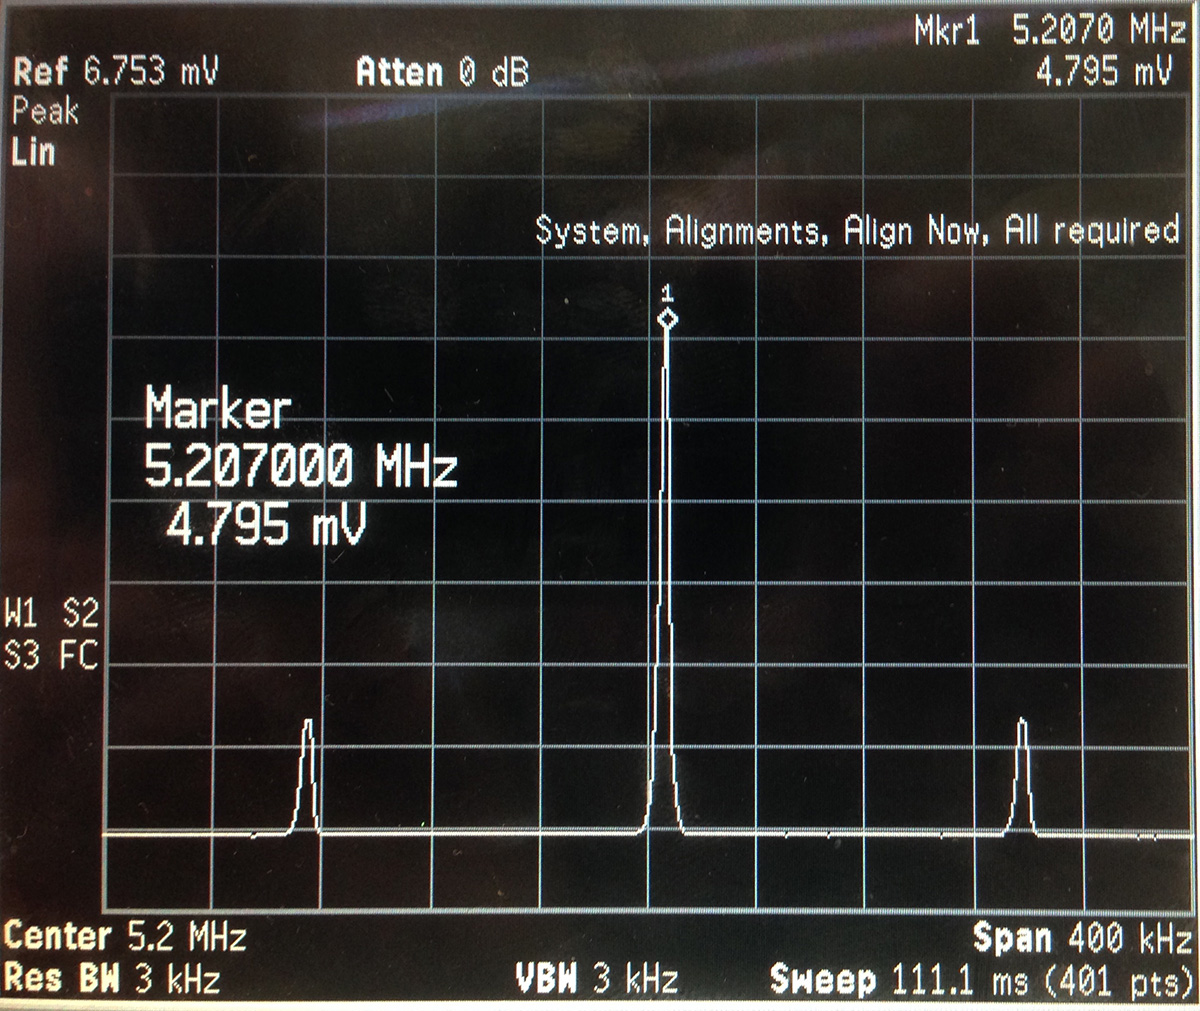
\includegraphics[width=0.8\linewidth]{images/am-diode-spektrum.jpg}
    \caption{
        Frequenzspektrum des mit Hilfe einer Diode erzeugten AM-Signals im
        Bereich um die Trägerfrequenz.
    }
    \label{fig:am-diode-spektrum}
\end{figure}
\begin{figure}
    \centering
    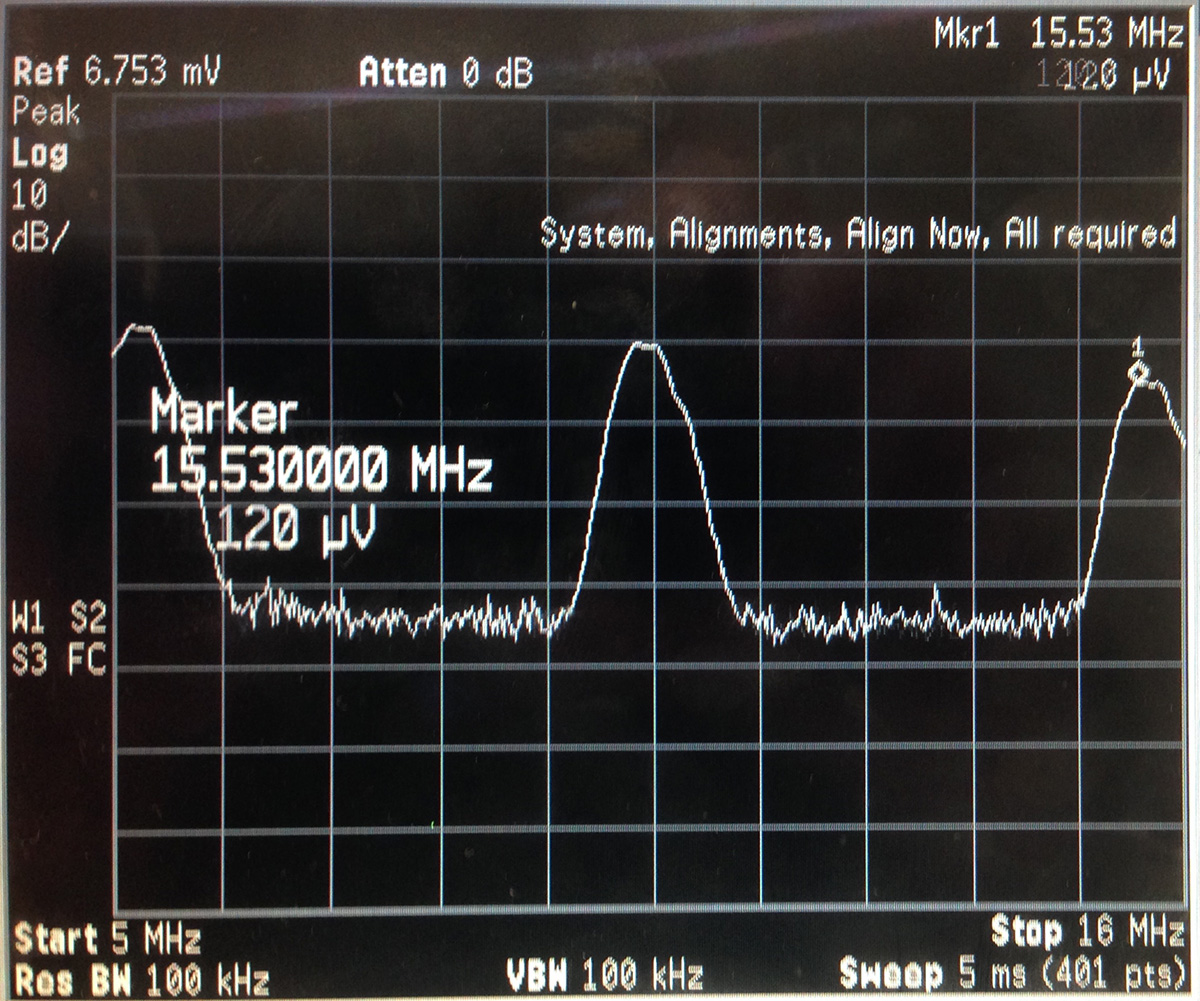
\includegraphics[width=0.8\linewidth]{images/am-diode-oberwellen.jpg}
    \caption{
        Oberwellen des AM-Singals.
    }
    \label{fig:am-diode-oberwellen}
\end{figure}

\subsubsection{Demodulation mit Ringmodulator}
\label{subsubsec:am-demodulation-ring}
Mit der in Abbildung XXX dargestellten Schaltung können AM-Signale mit
Kenntnis der Trägerspannung mit einem Ringmodulator demoduliert werden.
Zunächst wird die Abhängigkeit der Ausgangsspannung eines Ringmodulators
von der Phasendifferenz beider Eingangssignale untersucht. Dabei wird lediglich
eine Sinusspannung unterschiedlicher Laufzeit auf beide Eingänge gegeben.
Die Entsprechenden Messwerte sind in Tabelle \ref{tab:demodulation-cosinus}
aufgeführt und werden mitsamt einer Cosinus-Ausgleichsgerade in Abbildung
\ref{fig:demodulation-cosinus} dargestellt. Die Cosinus-Abhängigkeit ist
deutlich zu erkennen.
\begin{table}
    \centering
    \caption{Messwerte zur Bestimmung der Phasenabhängigkeit eines
    Ringmodulators}
    \label{tab:demodulation-cosinus}
    \begin{tabular}{SS@{\qquad}SS}
        \toprule
        {$T/\si{\nano\second}$} & {$U/\si{\milli\volt}$} & {$T/\si{\nano\second}$} & {$U/\si{\milli\volt}$} \\
        \midrule
         0 &   76 & 48 & -36 \\ 
         4 &   42 & 52 &  -4 \\ 
         8 &    8 & 56 &  13 \\ 
        12 &  -23 & 60 &  61 \\ 
        16 &  -58 & 64 &  95 \\ 
        20 &  -91 & 68 & 127 \\ 
        24 & -125 & 72 & 150 \\
        28 & -151 & 76 & 151 \\
        32 & -155 & 80 & 128 \\
        36 & -136 & 84 &  96 \\
        40 & -103 & 88 &  62 \\
        44 &  -70 & 92 &  30 \\
        \bottomrule
    \end{tabular}
\end{table}
\begin{figure}
    \centering
    \includegraphics[width=0.9\linewidth]{build/demodulation-cosinus.pdf}
    \caption{Phasenabhängigkeit eines Ringmodulators.}
    \label{fig:demodulation-cosinus}
\end{figure}

Wird anstelle eines Voltmeters ein Oszilloskop an den Ausgang des
Ringmodulators angeschlossen, kann das Eingangssignal fast unverändert
wiedererkannt werden.
Abbildung \ref{fig:am-demoduliert} stellt das Eingangssignal und das
demodulierte Signal nach einem Tiefpass in einem Bild dar.
Es ist zu erkennen, dass sich die Signale lediglich in einer Phase
und der Amplitude unterscheiden.
Das demodulierte Signal ohne Tiefpass ist in Abbildung \ref{fig:am-kein-tp}
dargestellt. Über die Cosinus-Schwingung legen sich hier einige höhere
Frequenzen.
\begin{figure}
    \centering
    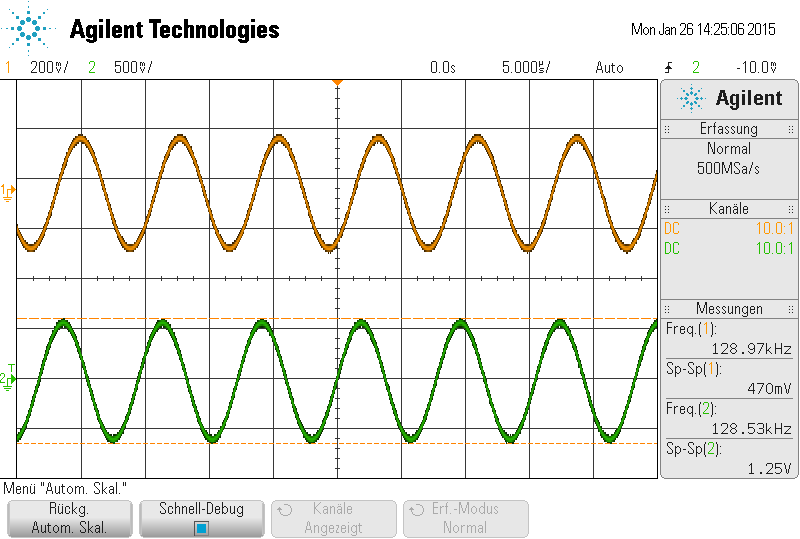
\includegraphics[width=0.8\linewidth]{images/am-demoduliert.png}
    \caption{Demodulation mit Ringmodulator. Reines (grün) und demoduliertes (gelb) Sinus-Signal nach
    Ringmodulator.}
    \label{fig:am-demoduliert}
\end{figure}
\begin{figure}
    \centering
    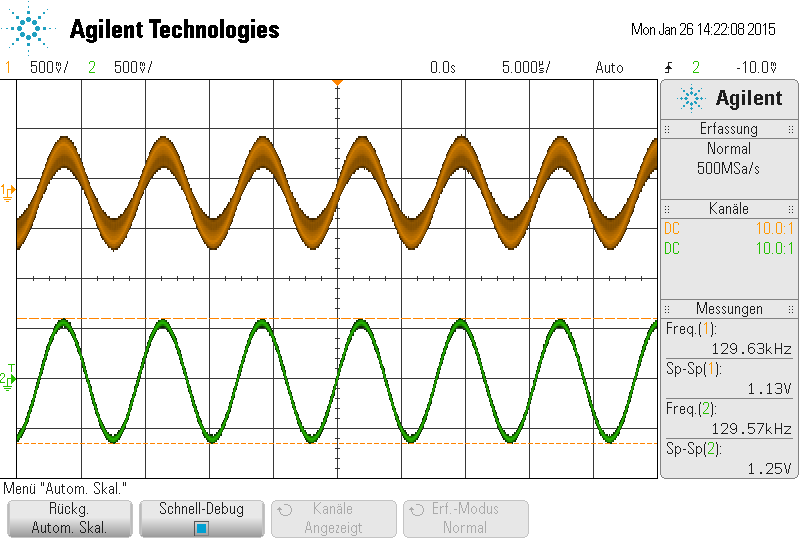
\includegraphics[width=0.8\linewidth]{images/am-kein-tp.png}
    \caption{Demodulation mit Ringmodulator. Reines (grün) und demoduliertes (gelb) Sinus-Signal hinter
    Ringmodulator ohne Tiefpass.}
    \label{fig:am-kein-tp}
\end{figure}

\subsubsection{Demodulation mit Gleichrichterdiode}
\label{subsubsec:gleichrichterdiode}
Mit Hilfe einer Gleichrichterdiode in einer Schaltung wie Abbildung
\ref{fig:dioden-schaltung} lassen sich AM-Signale ebenfalls demodulieren.
Auch hier steigert ein Tiefpass die Reinheit des Signals erheblich, wie
im Vergleich von Abbildungen \ref{fig:am-diode} und \ref{fig:am-diode-tp}
zu sehen ist.
\begin{figure}
    \centering
    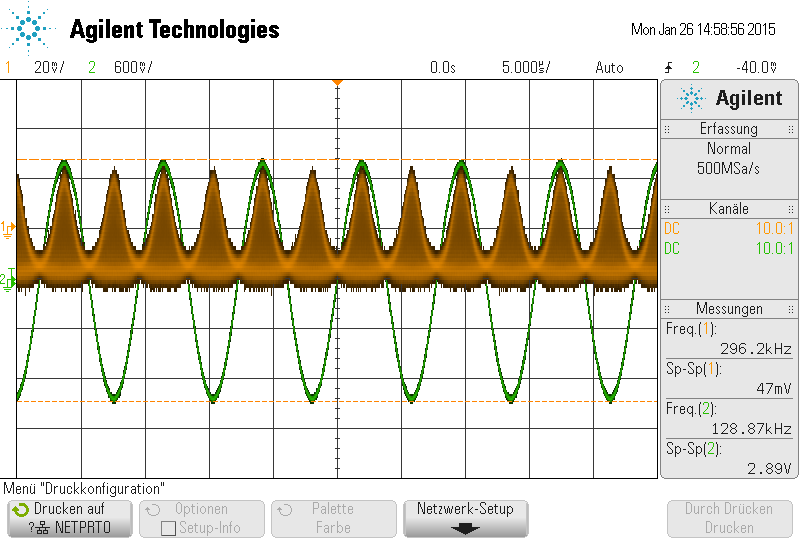
\includegraphics[width=0.8\linewidth]{images/am-diode.png}
    \caption{
        Demodulation mit Gleichrichterdiode.
        Demoduliertes Signal, genommen hinter Diode (gelb).
        Eingangssignal zum Vergleich (grün).
    }
    \label{fig:am-diode}
\end{figure}
\begin{figure}
    \centering
    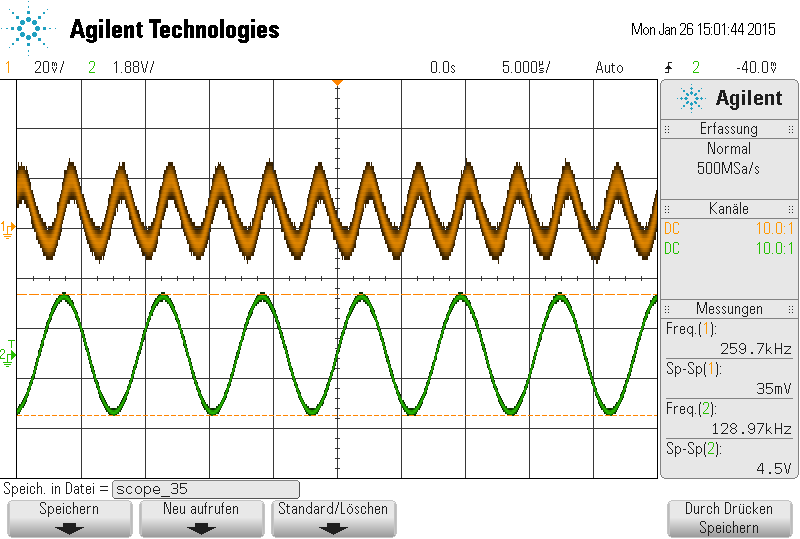
\includegraphics[width=0.8\linewidth]{images/am-diode-tp.png}
    \caption{
        Demodulation mit Gleichrichterdiode.
        Demoduliertes Signal, genommen hinter Tiefpass (gelb).
        Eingangssignal zum Vergleich (grün).
    }
    \label{fig:am-diode-tp}
\end{figure}

\subsection{Untersuchung an frequenzmodulierten Schwingungen}
\label{subsec:fm-auswertung}
In diesem Abschnitt wird eine frequenzmodulierte Schwingung erzeugt.
Dabei werden Frequenzhub und Modulationsgrad $m$ bestimmt, sowie
das Frequenzspektrum aufgenommen.

\subsubsection{Erzeugung einer frequenzmodulierten Schwingung}
\label{subsubsec:fm-erzeugung}
Zur Erzeugung einer FM-Schwingung wird hier die in Abbildung
\ref{fig:fm-erzeugung} Schaltung genutzt.
Um einen Phasenversatz von $\varphi = \pi/2$ zwischen Trägerspannung
$U_\text{T}$ und Ausgangssignal $U_3$ zu erlangen, muss die
Trägerfrequenz $\omega_\text{T}$ justiert werden.
Die beiden Spannungssignale ergeben bei richtiger Justage einen Kreis,
schließt man sie an X- und Y-Eingang eines Oszilloskopen an.
Das in Abbildung \ref{fig:fm-kreis} dargestellt Bild ergibt sich
bei einer Frequenz $\omega_\text{T} = \SI{0.981(1)}{\mega\hertz}$.
Die Trägerspannung beträgt dabei $U_\text{T} = \SI{4.50(3)}{\volt}$.
\begin{figure}
        \centering
        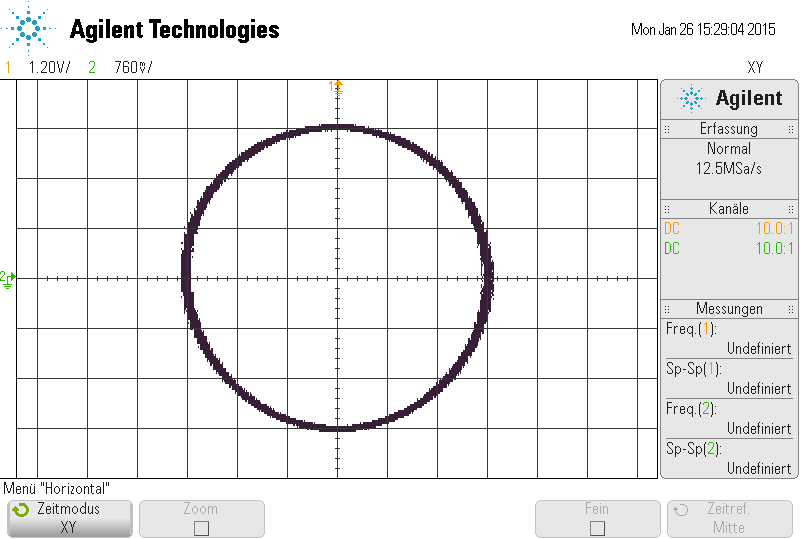
\includegraphics[width=0.8\linewidth]{images/fm-kreis.png}
        \caption{Lissajou-Figur von Trägerspannung $U_\text{T}$ und
        Ausgangsspannung $U_3$. Die Kreisform deutet auf eine Phase von
        $\varphi=\pi/2$ hin.}
        \label{fig:fm-kreis}
\end{figure}

Nachdem die Trägerfrequenz eingestellt ist, wird eine Modulationsspannung
hinzugeschaltet. Die Zeitabhängigkeit der modulierten Schwingung ist in
Abbildung \ref{fig:fm-zeitabh} dargestellt.
Die Modulationsfrequenz beträgt $\omega_\text{m} = \SI{164.6(5)}{\kilo\hertz}$,
die Spannung $U_\text{m} = \SI{2.94(3)}{\volt}$.
\begin{figure}
        \centering
        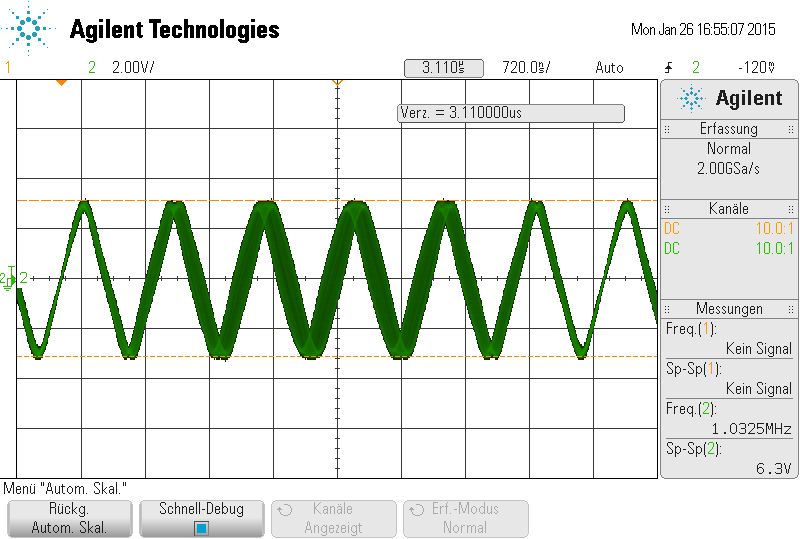
\includegraphics[width=0.8\linewidth]{images/fm-zeitabh.png}
        \caption{Frequenzmodulierte Spannung.}
        \label{fig:fm-zeitabh}
\end{figure}

\subsubsection{Frequenzhub und Modulationsgrad einer FM-Schwingung}
\label{subsubsec:fm-modulationsgrad}
Wie in Abbildung \ref{fig:fm-zeitabh} zu erkennen ist, verschmiert das
modulierte Signal periodisch.
Der Frequenzhub $\Delta f$ der Modulation lässt sich durch die Verbreiterung
der Periodendauern bestimmen.
Die Verbreiterung ist maximal nach drei Perioden und beträgt im Mittel
$\Delta T = \input{build/delta_t.tex}$ pro Periode. Mit der Periodendauer der
Trägerfrequenz $T_\text{T} = \input{build/t_t.tex}$ ergibt sich ein
Frequenzhub von $\Delta f = \input{build/delta_f.tex}$ und
damit der Modulationsgrad $m = \input{build/m.tex}$.
Die hierfür verwendeten Messwerte sind in Tabelle \ref{tab:delta_ts}
aufgeführt.
Abbildung \ref{fig:fm-spektrum} zeigt das Frequenzspektrum des Modulierten
Signals.
\begin{table}
        \centering
        \caption{Messwerte zur bestimmung des Frequenzhubs.}
        \label{tab:delta_ts}
        \begin{tabular}{S[table-format=1.0] S[table-format=4.0(1)] S[table-format=4.0(1)]}
                \toprule
                {Periode} & {$T_1 / \si{\nano\second}$} & {$T_2 / \si{\nano\second}$} \\
                \midrule
                1 &  960(5) & 1090(5) \\
                2 & 1940(5) & 2150(5) \\
                3 & 2940(5) & 3175(5) \\
                \bottomrule
        \end{tabular}
\end{table}
\begin{figure}
        \centering
        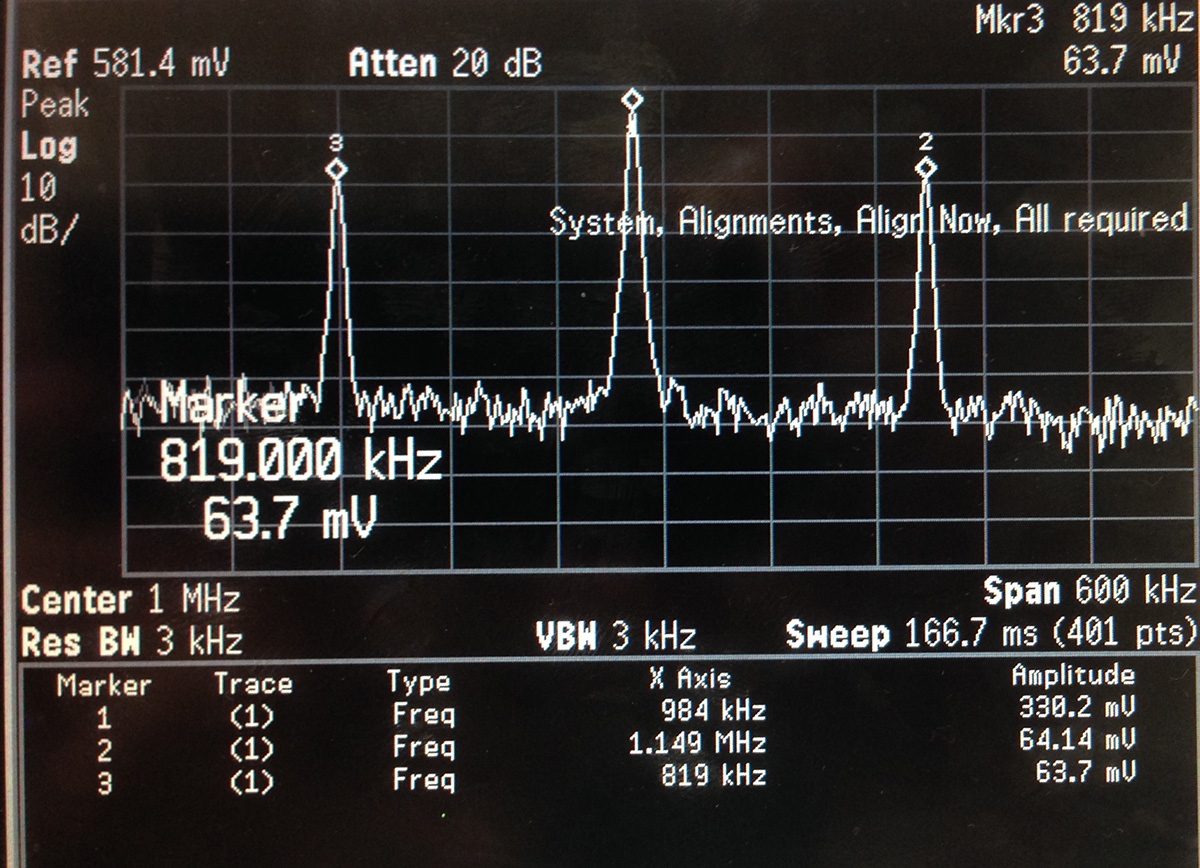
\includegraphics[width=0.8\linewidth]{images/fm-spektrum.jpg}
        \caption{Spektrum einer frequenzmodulierten Sinus-Schwingung.}
        \label{fig:fm-spektrum}
\end{figure}
